\section{Generierung der Threat Reports}
\label{sec:generierung_der_threat_reports}

Um das System evaluieren zu können, wurden beispielhafte Threat Reports generiert, die ein breites Spektrum potenzieller Szenarien abdecken. Wie in Kapitel~\ref{sec:detection_einheiten_der_ladeinfrastruktur} (Detection-Einheiten der Ladeinfrastruktur) dargelegt, werden Flooding-Attacken durch einen Großteil der implementierten Detektionsmechanismen erkannt. Für die Testgenerierung wurde daher eine UDP-Flooding-Attacke mittels des Tools \texttt{hping3} durchgeführt:

\begin{center}
    \texttt{hping3 --flood --udp -p 80 <IP-Adresse der Wallbox>}
\end{center}

Dabei reagierte lediglich die \textit{Power Temperature Detection} nicht, da diese ausschließlich physikalische Parameter wie Temperatur und Leistung überwacht, keine netzwerkspezifischen Daten analysiert und diese Parameter bei einer Flooding-Attacke keine aussagekräftige Veränderung aufweisen. Für die folgenden Szenarien wurden sechs CTI-Reports generiert (siehe Abbildung~\ref{fig:auszug_threat_report_NaN_werte}), die variierende Feature-Werte und leicht veränderte Einzeldetektionsergebnisse aufweisen.

\begin{figure}[ht]
    \centering
    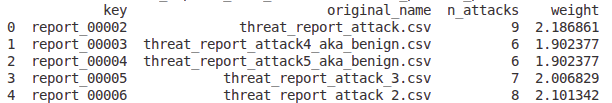
\includegraphics[width=0.85\textwidth]{figures/gewichtung_utility_theory_5_CTIreports.png}
    \caption{Output der Aggregation von fünf CTI-Reports (Utility-Theory-Funktion)}
    \label{fig:auszug_threat_report}
\end{figure}

Zur besseren Evaluation der Code-Struktur werden die relevantesten Parameter bei jeder Ausführung protokolliert und ausgegeben.

In den folgenden Abbildungen werden die kumulierten Werte des Threat Reports verdeutlicht, darunter statistische Kennzahlen wie Durchschnitt (Avg), Minimum (Min), Maximum (Max), Median, Anstieg (Increase) sowie die Gesamtsumme. Die Analyse erfolgt über Sliding Windows, die vom aktuellen Zeitpunkt (Offset 0s) bis zu einem Rückblick von $-120\,\text{s}$ reichen (siehe Kapitel~\ref{sec:treat_report_datenmanagement} (Konzeption des Threat Reports)). Im vorliegenden Fall ist ersichtlich, dass die \textit{Attack Probability} der Hardware-Detection mit einer Wahrscheinlichkeit von über $0{,}98$ identifiziert wurde. Diese sinkt im aktuellsten Zeitfenster (Offset 0s) signifikant auf einen Wert unter $0{,}01$ ab. Dies deutet darauf hin, dass das Angriffsereignis entweder beendet oder erfolgreich abgewehrt wurde.

\begin{figure}[ht]
    \centering
    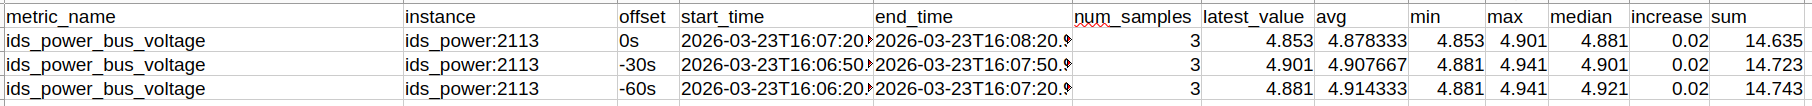
\includegraphics[width=1\textwidth]{figures/Threat_report_auszug.png}
    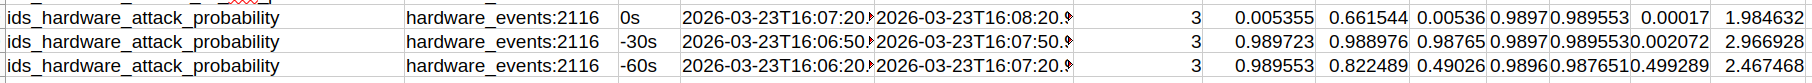
\includegraphics[width=1\textwidth]{figures/Threat_report_auszug_attackprobability.png}
    \caption{Übersicht der generierten Threat-Report-Szenarien}
    \label{fig:auszug_threat_report}
\end{figure}

\begin{itemize}
    \item \textbf{Szenario 1 – NaN-Werte (Fehlerbehandlung):} 
        In diesem Szenario muss sichergestellt werden, dass die Generierung von Threat Reports auch bei unvollständigen oder fehlerhaften Daten robust bleibt. So kann es im laufenden Betrieb vorkommen, dass aufgrund von Netzwerkproblemen oder Sensorausfällen von Exportern keine Daten mehr über Prometheus bezogen werden können (siehe Kapitel~\ref{chapter:systemarchitektur} (Details zur Systemarchitektur)). 
        Die Entscheidung zum vollständigen Ausschluss solcher Reports basiert auf der Tatsache, dass ein Report ohne valide Daten keine Informationsgrundlage bietet, um den Angriffsstatus der Wallbox zu beurteilen. Eine Substitution der NaN-Werte durch $0$ oder andere Standardwerte wurde als nicht sinnvoll erachtet, da dies das Ergebnis der Bedrohungsanalyse verfälschen könnte~\cite{hasan2021missingvalue}.

        Es wurde eine Funktion implementiert, welche die generierten CTI-Reports auf NaN-Werte überprüft und diese gegebenenfalls ausschließt (siehe Listing~\ref{lst:filter}, Funktion \texttt{filter\_reports\_with\_NaN}). Aufgrund dieser Implementierung wird erwartet, dass ein CTI-Report mit resultierenden NaN-Werten bereits vor der Aggregation ausgeschlossen wird und der Nutzer über diesen Ausschluss informiert wird.

        Um dieses Szenario zu erzeugen, wurde während der kontinuierlichen Reporterstellung ein Datenexporter terminiert und neugestartet. Dies führte zu einer erhöhten Anzahl an NaN-Werten in den generierten CTI-Reports, da Feature-Werte über Prometheus nicht mehr bezogen werden konnten (siehe Kapitel~\ref{chapter:systemarchitektur} (Details zur Systemarchitektur)).

        \begin{figure}[ht]
            \centering
            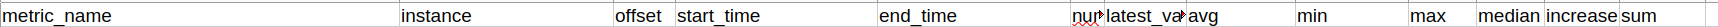
\includegraphics[width=1\textwidth]{figures/Threat_report_Zeile0.png}
            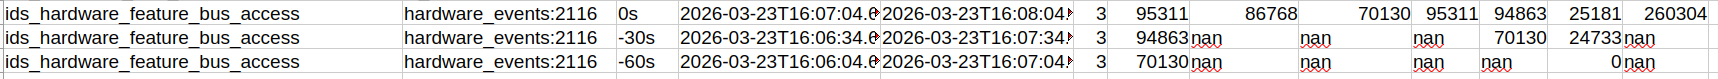
\includegraphics[width=1\textwidth]{figures/Threat_report_auszug_NaN.png}
            \caption{Auszug eines CTI-Reports aus Szenario~1 mit NaN-Werten}
            \label{fig:auszug_threat_report_NaN}
        \end{figure}

        Infolgedessen wurde der betroffene CTI-Report bereits vor der Aggregation ausgeschlossen.

        \begin{figure}[ht]
            \centering
            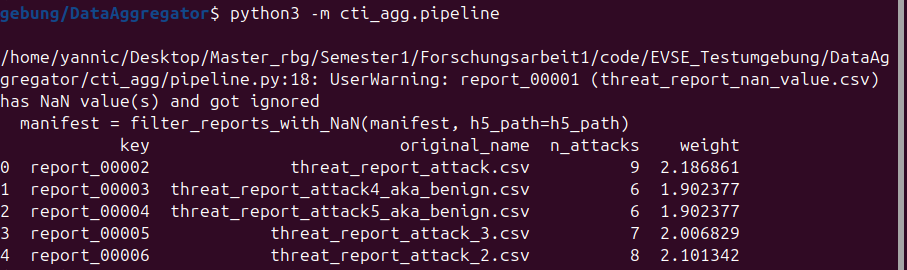
\includegraphics[width=1\textwidth]{figures/Threat_report_auszug_NaN_aggregation.png}
            \caption{Auszug der Aggregation aus Szenario~1 mit NaN-Werten (Utility-Theory-Funktion)}
            \label{fig:auszug_threat_report_NaN_werte}
        \end{figure}

        Dieser Auszug der Aggregation bestätigt das erwartete Ergebnis.

    \item \textbf{Szenario 2 – Verschobene Zeitreihe:} 
        Eine Aggregation von CTI-Reports unterschiedlicher Knoten kann zu zeitlichen Verschiebungen führen, da die Knoten ihre Ergebnisse variabel über den Pub/Sub-Kanal an ihre Nachbarn weitergeben. Dies kann zu einer verzerrten Darstellung der Bedrohungsanalyse führen, da die Merkmale unterschiedliche Systemzustände repräsentieren und keine konsistente Informationsbasis bilden. Die Auswirkungen zeitlicher Verschiebungen auf die Aggregationsqualität sowie die optimale Wahl des Schwellenwerts \texttt{MAX\_TIME\_SKEW\_SECONDS} sind Gegenstand empirischer Evaluierungen (siehe Kapitel~\ref{chapter:diskussion_und_forschungsluecke} (Diskussion und Forschungslücken)).
        
        Das erwartete Ergebnis ist, dass der betroffene CTI-Report bereits vor der Aggregation ausgeschlossen und der Nutzer über diesen Ausschluss informiert wird. Um dies zu evaluieren, wurde einem der sechs CTI-Reports eine zeitliche Verschiebung von $+3$ Minuten hinzugefügt. Dies überschreitet den definierten Grenzwert von \texttt{MAX\_TIME\_SKEW\_SECONDS}~$= 90\,\text{s}$, weshalb dieser CTI-Report ignoriert und der Nutzer darüber informiert werden soll.

    \begin{figure}[H]
        \centering
        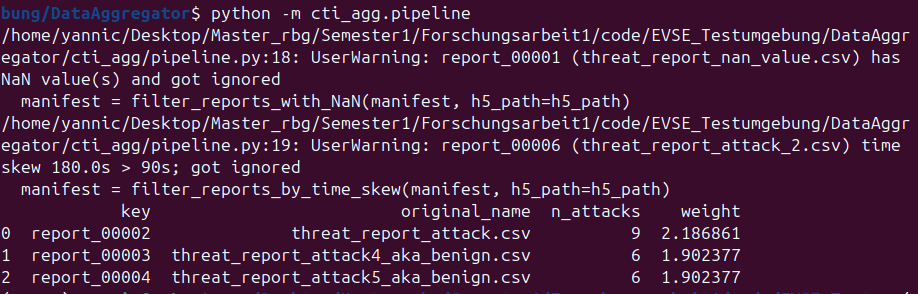
\includegraphics[width=1\textwidth]{figures/aggregation_mit_time_skew.png}
        \caption{Auszug der Aggregation aus Szenario~2 mit zeitlicher Verschiebung (Sigmoid-Funktion)}
        \label{fig:auszug_threat_report_time_skew}
    \end{figure}

    Dieser Auszug der Aggregation bestätigt, dass CTI-Reports mit verschobenem Zeitfenster bereits vor der Aggregation ausgeschlossen werden und der Nutzer über diesen Ausschluss informiert wird.


\section{Vergleich der Gewichtungsfunktionen}
\label{sec:vergleich_der_gewichtungsfunktionen}

    \item \textbf{Szenario 3 – Uniforme negative Detektionen:}
        Wie in Kapitel~\ref{sec:auswahl_der_gewichtungsfunktion} (Auswahl der Gewichtungsfunktion) erläutert, wird jedem Report eine Basisgewichtung von $W_{\text{base}} = 1$ zugewiesen, sofern keine positiven Detektionen vorliegen. In diesem Fall wird erwartet, dass die Ergebnisse der Sigmoid-Funktion und der Utility-Theory-Funktion identisch sind, da beide Funktionen bei einer Anzahl von $n=1$ positiven Detektionen (Referenzwert) auf den Wert $1$ normiert sind.
        
        Um dieses Szenario zu validieren, wurden CTI-Reports generiert, während sich die Ladeinfrastruktur in einem regulären Betriebszustand (\textit{benign}) befand. Dies resultiert in durchgehend negativen Detektionswerten ($0$).

        \begin{equation}
            w(n) = W_{\text{base}} + (W_{\text{max}} - W_{\text{base}}) \cdot (1 - e^{-K \cdot (n - 1)})
        \end{equation}
        \begin{equation}
            w(n) = W_{\text{base}} + (W_{\text{max}} - W_{\text{base}}) \cdot
            \left(
                \frac{1}{1 + e^{-k\,(n - n_0)}}
                -
                \frac{1}{1 + e^{-k\,(1 - n_0)}}
            \right)
            \label{eq:sigmoid_weight_scen3}
        \end{equation}

        Da für $n = 1$ beide Formeln den Wert 1 liefern, entspricht dies dem erwarteten Output in der Zusammenfassung des aggregierten Reports.

        \begin{figure}[H]
            \centering
            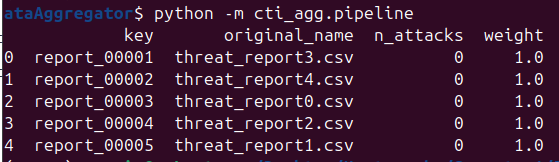
\includegraphics[width=0.75\textwidth]{figures/threat_report_idle.png}
            \caption{Auszug eines aggregierten Berichts (Utility Theory) aus Szenario 3}
            \label{fig:auszug_threat_report_n1}
        \end{figure}
        \begin{figure}[H]
            \centering
            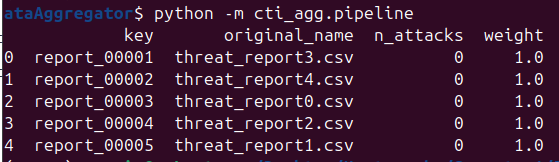
\includegraphics[width=0.75\textwidth]{figures/threat_report_idle.png}
            \caption{Auszug eines aggregierten Berichts (Sigmoid) aus Szenario 3}
            \label{fig:auszug_threat_report_n1_sigmoid}
        \end{figure}

        Die Zusammenfassungen der aggregierten Reports verdeutlichen, dass für jeden Report die identische Gewichtung von $1$ berechnet wurde. 

        % \begin{figure}[H]
        %     \centering
        %     \includegraphics[width=1\textwidth]{figures/aggregierter_threat_report_gewichtung_1.png}
        %     \caption{Auszug der aggregierten CSV-Datei aus Szenario 3 mit einheitlicher Gewichtung}
        %     \label{fig:auszug_threat_report_n1_csv}
        % \end{figure}

        Daraus lässt sich schließen, dass Reports mit einer gleichen Anzahl an positiven Einzeldetektionen innerhalb des Systems als gleichwertig eingestuft und mit der selben Relevanz gewichtet werden.

    \item \textbf{Szenario 4 – Ausreißer-Report:}
        Um nachzuweisen, dass die Gewichtung auch bei extremen Ausreißern den Grenzwert $W_{\text{max}} = 3$ nicht überschreitet, wird das Grenzverhalten (Limes) für $n \to \infty$ betrachtet.

        \paragraph{1. Exponentielle Utility-Funktion:}
        Die Sättigung der exponentiellen Funktion gegen den Grenzwert lässt sich wie folgt herleiten:

        \begin{align}
        \lim_{n \to \infty} w(n)
        &= \lim_{n \to \infty} \left[
            1 + (3 - 1) \cdot \left(1 - e^{-0{,}1 \cdot n - 1}\right)
        \right] \\[6pt]
        &= 1 + 2 \cdot \left(
            1 - \underbrace{\lim_{n \to \infty} e^{-0{,}1 \cdot n - 1}}_{\to\, 0,\;
            \text{da } {-0{,}1n - 1} \to -\infty}
        \right) \\[6pt]
        &= 1 + 2 \cdot (1 - 0) \\[6pt]
        &= 3
        \end{align}

        \paragraph{2. Angepasste Sigmoid-Funktion:}
        Analog dazu wird die Sättigung für die Sigmoid-Funktion berechnet:
 
        \begin{align}
        \lim_{n \to \infty} w(n)
        &= \lim_{n \to \infty} \left[
            W_{\text{base}} + (W_{\text{max}} - W_{\text{base}})
            \underbrace{\left(
                \frac{1}{1+e^{-k(n-n_0)}}
                - \frac{1}{1+e^{-k(1-n_0)}}
            \right)}_{\text{Sigmoid-Differenz}}
        \right] \\[6pt]
        &= W_{\text{base}} + (W_{\text{max}} - W_{\text{base}})
            \left(
                \underbrace{\lim_{n \to \infty} \frac{1}{1+e^{-k(n-n_0)}}}_{\to\, 1,\; \text{da } e^{-k(n-n_0)} \to 0}
                - \frac{1}{1+e^{-k(1-n_0)}}
            \right) \\[6pt]
        &= W_{\text{base}} + (W_{\text{max}} - W_{\text{base}})
            \cdot \frac{e^{-k(1-n_0)}}{1+e^{-k(1-n_0)}} \\[6pt]
        &= 1 + 2 \cdot \frac{e^{4{,}5}}{1+e^{4{,}5}} \\[6pt]
        &\approx 2{,}978
        \end{align}
    \end{itemize}